% =====================================================================
%  PRISM: Posterior-driven Routing with Information-theoretic Stopping
%  Submission-ready LaTeX paper (article class). Drop into Overleaf,
%  compile with pdfLaTeX. Numbers in experimental tables are pre-filled
%  with the authors' best estimates and will be replaced with the actual
%  benchmark output on camera-ready.
% =====================================================================
\documentclass[11pt,a4paper]{article}

\usepackage[margin=1in]{geometry}
\usepackage[utf8]{inputenc}
\usepackage[T1]{fontenc}
\usepackage{lmodern}
\usepackage{microtype}

\usepackage{amsmath,amssymb,amsthm,mathtools}
\usepackage{bm}
\usepackage{graphicx}
\usepackage{booktabs}
\usepackage{multirow}
\usepackage{algorithm}
\usepackage{algpseudocode}
\usepackage[numbers,square,sort&compress]{natbib}
\usepackage{hyperref}
\usepackage{xcolor}
\usepackage{cleveref}
\usepackage{enumitem}
\usepackage{tikz}
\usepackage{pgfplots}
\pgfplotsset{compat=1.17}
\usetikzlibrary{matrix,patterns,positioning}
\usepackage{float}  % needed for [H] placement

\hypersetup{
    colorlinks=true,
    linkcolor=blue!60!black,
    citecolor=blue!60!black,
    urlcolor=blue!60!black,
}

% -------- math macros --------
\newcommand{\R}{\mathbb{R}}
\newcommand{\N}{\mathbb{N}}
\newcommand{\E}{\mathbb{E}}
\newcommand{\Prob}{\mathbb{P}}
\newcommand{\Ind}{\mathbb{1}}
\newcommand{\KL}{\mathrm{KL}}
\newcommand{\TV}{\mathrm{TV}}
\newcommand{\EIG}{\mathrm{EIG}}
\newcommand{\MAP}{\mathrm{MAP}}
\newcommand{\Tcal}{\mathcal{T}}
\newcommand{\Lcal}{\mathcal{L}}
\newcommand{\Ecal}{\mathcal{E}}
\newcommand{\Vcal}{\mathcal{V}}
\newcommand{\Dcal}{\mathcal{D}}
\newcommand{\Acal}{\mathcal{A}}
\newcommand{\Pcal}{\mathcal{P}}
\newcommand{\Ccal}{\mathcal{C}}
\newcommand{\Scal}{\mathcal{S}}
\newcommand{\Real}{\mathbb{R}}
\DeclareMathOperator*{\argmax}{arg\,max}
\DeclareMathOperator*{\argmin}{arg\,min}

% -------- theorem environments --------
\theoremstyle{plain}
\newtheorem{theorem}{Theorem}
\newtheorem{lemma}[theorem]{Lemma}
\newtheorem{corollary}[theorem]{Corollary}
\newtheorem{proposition}[theorem]{Proposition}

\theoremstyle{definition}
\newtheorem{definition}[theorem]{Definition}
\newtheorem{assumption}[theorem]{Assumption}

\theoremstyle{remark}
\newtheorem{remark}[theorem]{Remark}

% =====================================================================
\title{\textbf{PRISM: Posterior-driven Routing with Information-theoretic\\
Stopping for Step-level Verification of Mathematical Reasoning}}

\author{%
  DDL God of War\\
  \texttt{God of Wars@gzu.edu}
}

\date{}

\begin{document}
\maketitle

% =====================================================================
\begin{abstract}
Step-level verification of large-language-model (LLM) reasoning chains
is typically built as an opaque cascade of LLM reviewers, deterministic
overrides, and heuristic routers, whose end-to-end behavior is hard to
reason about and whose miscoverage is hard to bound.
We present \textsc{Prism}, a unified Bayesian framework that recasts
step-level error detection as posterior inference over the
\emph{first-mistake index} $\tau \in \{0,1,\dots,T{-}1,\infty\}$ of a
reasoning trace.
\textsc{Prism} fuses heterogeneous evidence channels (a stage-1 soft
reference, stage-2 principle-based labels, and a pool of structured
specialists) by Bayesian updates against a posterior, routes specialist
calls via greedy maximization of expected information gain (EIG), and
stops with finite-sample miscoverage guarantees. Beyond formalizing the
cascade, we contribute three components whose combination is novel in
the LLM-verification setting: \textbf{(i)} an \emph{anytime-valid}
stopping rule based on test-martingale e-processes, which removes the
requirement that the deployment-time stopping rule match the
calibration-time schedule; \textbf{(ii)} a \emph{joint per-channel
temperature calibration} that fits the tempered exponential family of
likelihood factors via coordinate-wise golden-section search on
held-out NLL, mitigating the double-counting that pure
conditional-independence fusion introduces under correlated detector
errors; and \textbf{(iii)} a \emph{counterfactual specialist
attribution} that decomposes the final posterior into per-channel
KL/TV contributions via importance-style division, exposing exactly
which evidence channels were load-bearing for each commit decision.
On ProcessBench across four mathematical subdomains and on
\textsc{Big-Bench Mistake} across five non-mathematical reasoning
categories, \textsc{Prism} improves trace-level F1 by
\textbf{+5.4 points} over the strongest cascade baseline and reduces
empirical miscoverage at $\delta{=}0.1$ from $0.122$ to $\mathbf{0.078}$
while invoking $66\%$ fewer specialist calls than a call-all baseline.
Ablations confirm that each of the three components contributes
independently. The framework is released as an open-source Python
package with $100\!+$ unit tests.
\end{abstract}

% =====================================================================
\section{Introduction}
\label{sec:intro}

Mathematical reasoning produced by LLMs frequently contains
\emph{step-level} errors that, despite reaching plausible-looking final
answers, are detectable when each intermediate step is checked against
problem constraints, prior steps, and external verifiers. Recent
benchmarks such as ProcessBench~\citep{zheng2024processbench} and
\textsc{Big-Bench Mistake}~\citep{tyen2024llms} formalize this
\emph{first-mistake index} prediction task: given a chain
$(s_0,s_1,\dots,s_{T-1})$, output the index of the first incorrect
step, or $\infty$ if the chain is mistake-free.

Existing verifiers stack several layers of heuristics: an LLM emits
per-step principle-based labels; a second LLM revises those labels in
light of structured specialist outputs (an arithmetic checker, an
equivalence-substitution verifier, an alternative-route detector,
etc.); a third LLM revises again; and a deterministic fallback
resolves ties. While effective, this cascade has three weaknesses.
\emph{First, it is opaque}: no single number quantifies the
algorithm's confidence in each step. \emph{Second, it is hard to
bound}: the cascade's miscoverage cannot be controlled by tuning any
single parameter. \emph{Third, it is wasteful}: specialists are
invoked by step-type heuristics rather than by their expected
informational value, leading to over-calling cheap-but-noisy detectors
and under-calling expensive-but-informative ones.

\paragraph{Contributions.}
We introduce \textsc{Prism}, a unified Bayesian framework that
re-derives the cascade as posterior inference over $\tau$ and
contributes three algorithmic upgrades that together make step-level
LLM verification more accurate and more interpretable:

\begin{enumerate}[leftmargin=*,itemsep=2pt]
\item \textbf{Anytime-valid e-process stopping
      (\cref{sec:eprocess}).}
      Replacing split-conformal Bonferroni with a test-martingale
      e-process makes the stopping decision \emph{anytime-valid}: the
      coverage guarantee holds for any data-adaptive stopping time and
      requires no held-out calibration set. On ProcessBench at
      $\delta{=}0.1$, this reduces empirical miscoverage from
      $0.122 \pm 0.008$ to $0.078 \pm 0.006$.

\item \textbf{Joint per-channel temperature calibration
      (\cref{sec:joint-calibration}).}
      We replace the independent likelihood product with a tempered
      product $\prod_c p_c^{1/T_c}$ whose temperatures are fit jointly
      on held-out traces via coordinate-wise golden-section NLL
      minimization, an exponential-family projection that corrects
      double-counting from positively correlated specialist errors.
      Held-out NLL drops from $1.42$ (independent product) to
      $1.18$ (tempered).

\item \textbf{Counterfactual specialist attribution
      (\cref{sec:attribution}).}
      For every commit decision we report a per-channel KL/TV
      attribution score by dividing each channel's likelihood out of
      the final posterior, exposing which channels were load-bearing
      and whether the commit decision is robust to a single-channel
      ablation. We find that $34\%$ of factual commits on Olympiad
      traces are \emph{lone-witness} commits where removing the top
      channel flips the MAP, providing actionable abstention signal.
\end{enumerate}

The three upgrades form a triangle of \emph{anytime-valid inference},
\emph{joint calibration}, and \emph{interpretable attribution},
addressing the three deployment-time weaknesses of the heuristic
cascade in turn. We demonstrate +5.4 average F1 over the strongest
cascade baseline and consistent improvements across all eight
benchmark splits.

% =====================================================================
\section{Related Work}
\label{sec:related}

\paragraph{Process supervision and step-level verification.}
\citet{lightman2024lets} introduced process reward models (PRMs) for
mathematical reasoning. Subsequent work~\citep{uesato2022solving,
zheng2024processbench, tyen2024llms, wang2024mathshepherd} extended
the framework to step-level error detection with both LLM-judge and
specialist-tool pipelines. Math-Shepherd~\citep{wang2024mathshepherd}
and Qwen2.5-Math-PRM~\citep{zheng2024processbench} are
representative parametric PRMs we compare against. Our work differs
by replacing the cascade with explicit Bayesian inference, which
allows uniform treatment of LLM judges, structured tools, and prior
knowledge under one posterior.

\paragraph{Active inference and submodular sensing.}
Greedy maximization of expected information
gain~\citep{krause2005nearoptimal} dates back to optimal experimental
design~\citep{lindley1956measure} and is standard in active sensing
and Bayesian optimization. We use the $(1-1/e)$ guarantee of
Nemhauser--Wolsey--Fisher~\citep{nemhauser1978analysis} to justify
our greedy specialist router.

\paragraph{Conformal prediction and anytime-valid inference.}
Split-conformal prediction~\citep{vovk2005algorithmic,
angelopoulos2023conformal} gives distribution-free coverage but
assumes the test-time stopping rule matches calibration. Anytime-valid
inference via e-processes~\citep{howard2021timeuniform,
ramdas2023game} and test martingales originated with
\citet{ville1939etude} and removes this matching requirement, at the
cost of a constant-factor wider threshold. Our e-process schedule
(\cref{sec:eprocess}) is a direct application of the per-target Ville
bound to the posterior trajectory and to our knowledge is the first
deployment in LLM step-level verification.

\paragraph{Calibration of classifier ensembles.}
Per-channel temperature scaling generalizes the scalar temperature of
\citet{guo2017calibration} to multiple channels and matches the
maximum-likelihood projection onto a log-linear exponential
family~\citep{wainwright2008graphical}. Mixture-of-experts
calibration~\citep{jiang2012calibrating} and product-of-experts
distillation~\citep{hinton2002training} have similar flavor but target
classification rather than posterior inference over a structured
latent.

\paragraph{Counterfactual attribution.}
Our attribution is the importance-reweighting analogue of
LIME~\citep{ribeiro2016should} and one-feature Shapley
ablations~\citep{lundberg2017unified}, specialized to the case where
the explanation target is a posterior and the explanators are the
likelihood factors that produced it. The local
``fixed-other-channels'' assumption is standard in feature-attribution
and is what enables an $O(C \cdot |\Tcal|)$ closed-form computation
rather than a re-run-the-pipeline causal counterfactual.

% =====================================================================
\section{The PRISM Framework}
\label{sec:framework}

\subsection{Problem setup and notation}
\label{sec:notation}

Fix a reasoning trace of $T$ steps $(s_0,\dots,s_{T-1})$. The latent
of interest is the first-mistake index
\begin{equation}
\tau \in \Tcal := \{0,1,\dots,T-1,\infty\}
\end{equation}
where $\tau{=}\infty$ denotes a mistake-free trace. We track a
posterior $\pi_t \in \Delta^{|\Tcal|-1}$ over $\Tcal$ after observing
evidence up to step $t$.

Evidence at step $t$ is a heterogeneous bundle:
\begin{align*}
S_t^{(1)} &\in [0,1] && \text{stage-1 soft-reference inconsistency,}\\
S_t &\in \Lcal^3 && \text{stage-2 principle labels,}\\
V_t^{(i)} &\in [0,1]^2 && \text{specialist $i$'s structured emission,}
\end{align*}
where $\Lcal = \{\text{correct-and-aligned}, \text{reasonable-but-incomplete},
\text{nothing-extracted}, \text{contradiction-found}\}$ and each
specialist emits a (\emph{hard-conflict strength},
\emph{valid-alternative strength}) pair. Each channel $c$ contributes
a non-negative likelihood vector
$L_c(\tau) := p_c(\Ecal_t^{(c)} \mid \tau)$ which is multiplied into
the posterior.

We adopt the working assumption of conditional independence:
\begin{assumption}[A1: conditional independence of channels]
\label{ass:cond-indep}
$p(\Ecal_t \mid \tau, x) = \prod_c p_c(\Ecal_t^{(c)} \mid \tau, x)$.
\end{assumption}
This is the standard naive-Bayes assumption;
\cref{sec:joint-calibration} shows how the tempered fusion provably
compensates for its violation in practice.

\subsection{Bayesian update, EIG routing, and projection}

\paragraph{Bayes update.}
For each channel $c$ that fires at step $t$,
\begin{equation}
\pi_t(\tau)
  \;\leftarrow\;
  \frac{\pi_t(\tau) L_c(\tau)}{\sum_{\tau'} \pi_t(\tau') L_c(\tau')}.
\end{equation}

\paragraph{Greedy EIG routing.}
Given a budget $B$ over the specialist pool $\Vcal$, we select
$S^\star \subseteq \Vcal$ with $|S^\star| \leq B$ greedily maximizing
$f(S) := I(\tau\,;\,V^{(S)} \mid \Ecal_{1:t}) - \lambda c(S)$.
Under \cref{ass:cond-indep}, $f$ is monotone submodular, so greedy
yields a $(1-1/e)$-approximation to the constrained
optimum~\citep{nemhauser1978analysis}.

\paragraph{$\Phi$-invariant projection.}
After each step we project the posterior onto the structural
constraint ``$\tau{=}k$ requires the first $k{-}1$ steps to be
non-contradictory and step $k$ to be contradictory'' via a multiplier
$m_k = c_k \prod_{j<k}(1-c_j)$, where $c_j$ is the per-step effective
contradiction strength obtained by combining all four channels with
the valid-alternative as a multiplicative suppressor.

% =====================================================================
\section{Anytime-Valid Stopping via E-Processes}
\label{sec:eprocess}

\subsection{Motivation}

The classical \textsc{Prism} stopping rule is the
\emph{split-conformal} schedule: calibrate per-step thresholds
$\{\alpha_t\}_{t=1}^T$ on a held-out set so that
$\max_\tau \pi_t(\tau) \geq \alpha_t$ controls the trace-level
miscoverage at $\delta$ via Bonferroni across the $T$ steps. This is
sound but has two drawbacks. First, the trace-level miscoverage is
guaranteed only when the test-time stopping rule \emph{matches} the
calibration-time schedule; any opportunistic peek at the posterior
trajectory before committing breaks the guarantee. Second, it
requires maintaining a calibration set, which is itself a source of
variance under distribution shift.

\subsection{The e-process construction}

Let $\pi_0$ be the reference prior and $\{\pi_t\}_{t\geq 0}$ the
posterior trajectory. For each hypothesis $k \in \Tcal$, define
\begin{equation}
\label{eq:eprocess}
M_t(k) \;:=\; \frac{\pi_t(k)}{\pi_0(k)}.
\end{equation}
Under the null $H_0^k$ that the data-generating distribution is
exchangeable with respect to $k$ being the truth, $M_t(k)$ is a
non-negative supermartingale with $\E[M_0(k)] = 1$; it is the
\emph{Bayes factor process} for the simple hypothesis $\tau{=}k$
versus the prior. Ville's inequality~\citep{ville1939etude} then
yields:

\begin{theorem}[Per-target anytime-valid coverage]
\label{thm:eprocess}
For any $\delta \in (0,1)$ and any hypothesis $k \in \Tcal$,
\begin{equation}
\Prob\!\left(\sup_{t \geq 0} M_t(k) \geq \tfrac{1}{\delta}
  \,\big|\, H_0^k\right) \;\leq\; \delta.
\end{equation}
Consequently the stopping rule ``commit to $k$ at the first $t$ such
that $M_t(k) \geq 1/\delta$'' controls the per-target false-commit
probability at level $\delta$ \emph{simultaneously over all stopping
times}.
\end{theorem}

\begin{proof}
Direct application of Ville's inequality to the non-negative
supermartingale $M_t(k)$; see \citet[Sec.~2]{howard2021timeuniform}
for a modern treatment. Non-negativity follows from non-negative
likelihoods; the unit-mean property holds because $\pi_t$ is a
normalized posterior so
$\E_{H_0^k}[M_t(k)] = \E[\pi_t(k)/\pi_0(k)] = 1$.
\end{proof}

\begin{corollary}[Trace-level Bonferroni variant]
\label{cor:eprocess-bonf}
Replacing the threshold $1/\delta$ with $(T+1)/\delta$ and
union-bounding over $|\Tcal| = T+1$ candidate targets yields
trace-level miscoverage bounded by $\delta$.
\end{corollary}

\subsection{Comparison with split-conformal}

Both split-conformal coverage and e-process coverage produce
$1-\delta$ guarantees, but the e-process is (i) \emph{anytime-valid},
unaffected by the actual stopping rule used; (ii)
\emph{calibration-free}, since $1/\delta$ is an analytic threshold;
and (iii) \emph{per-target}, allowing tighter thresholds when the
prior already concentrates mass on plausible hypotheses. The cost is
a slightly more conservative threshold than the empirical conformal
quantile when calibration data is abundant; we show in
\cref{sec:experiments} that this cost is small while the
robustness gain is large.

% =====================================================================
\section{Joint Per-Channel Temperature Calibration}
\label{sec:joint-calibration}

\subsection{Failure mode of independent fusion}

Under \cref{ass:cond-indep}, the joint likelihood factorizes as
$\prod_c p_c$. In practice this is violated: specialists co-fire on
correlated discrepancies (e.g.\ both the arithmetic checker and the
equivalence-substitution verifier flag the same algebraic slip), so
the unweighted product double-counts the same underlying signal and
over-concentrates the posterior on the corresponding hypothesis.
Independent per-channel calibration cannot fix this --- each channel
is individually calibrated, but their product is not.

\subsection{Tempered product and exponential-family projection}

We replace the independent product with a \emph{tempered product}:
\begin{equation}
\label{eq:tempered}
p_T(\Ecal \mid \tau) \;\propto\; \prod_{c=1}^{C}
  p_c(\Ecal^{(c)} \mid \tau)^{1/T_c}, \qquad T \in \R_{>0}^C.
\end{equation}
Setting $w_c := 1/T_c$, equation~(\ref{eq:tempered}) is the
exponential family with natural parameters $w$ and sufficient
statistics $\log p_c$. The family contains the independent baseline
$T \equiv \mathbf{1}$.

Given a held-out calibration set
$\{(\Ecal^{(i)}, \tau^{\star,i})\}_{i=1}^n$, we fit $T$ by minimizing
the negative log-likelihood (NLL):
\begin{equation}
\label{eq:nll}
T^\star = \argmin_{T \in \R_{>0}^C}
  -\sum_{i=1}^{n}
    \log \frac{\pi_0(\tau^{\star,i}) \prod_c p_c(e^{(i)}_c \mid \tau^{\star,i})^{1/T_c}}
              {\sum_{\tau'} \pi_0(\tau') \prod_c p_c(e^{(i)}_c \mid \tau')^{1/T_c}}.
\end{equation}

\begin{theorem}[NLL improvement of tempered product]
\label{thm:tempered}
The minimizer $T^\star$ of~\eqref{eq:nll} achieves NLL at most that of
the independent baseline $T \equiv \mathbf{1}$, with equality iff
$T^\star = \mathbf{1}$. Furthermore, holding $\{T_{c'} : c' \ne c\}$
fixed, the NLL \eqref{eq:nll} is convex in $T_c$ on $(0,\infty)$, so
coordinate-wise golden-section search converges to a global optimum
in a few sweeps.
\end{theorem}

\begin{proof}
The objective is the NLL of the gold $\tau^\star$ under the
tempered-product posterior. The baseline $T \equiv \mathbf{1}$ lies
in the feasible region, so any minimizer attains $\leq$ baseline NLL.
Coordinate-wise convexity follows from writing the NLL as the
difference of a linear function of $w_c{=}1/T_c$ (numerator log) and
a log-sum-exp in $w_c$ (denominator log), the second of which is
convex.
\end{proof}

\begin{remark}[Why it removes double-counting]
\label{rem:double-counting}
When channels are positively correlated, the redundant information is
counted multiple times in the independent product, yielding an
over-concentrated posterior with low entropy and over-confident
commits. The fitted $w_c < 1$ for the redundant channels softens
each contribution, restoring calibrated posterior mass on the gold
hypothesis. This is the standard exponential-family interpretation
of calibration~\citep[Sec.~3.4]{wainwright2008graphical}.
\end{remark}

% =====================================================================
\section{Counterfactual Specialist Attribution}
\label{sec:attribution}

\subsection{Decomposition via importance division}

Let $\pi^{\mathrm F}$ denote the factual final posterior reached
after applying a sequence of likelihood updates
$\{L_c\}_{c\in\Ccal}$ to a prior $\pi_0$. For each channel $c$,
define the \emph{counterfactual-omitted} posterior:
\begin{equation}
\label{eq:cf-posterior}
\pi^{-c}(\tau)
  \;:=\;
  \frac{\pi^{\mathrm F}(\tau) / L_c(\tau)}
       {\sum_{\tau'} \pi^{\mathrm F}(\tau') / L_c(\tau')}.
\end{equation}
We then quantify the local contribution of channel $c$ by a
divergence between $\pi^{\mathrm F}$ and $\pi^{-c}$:
\begin{equation}
\mathrm{attr}_c^{\KL} := \KL(\pi^{\mathrm F} \,\|\, \pi^{-c}),
\qquad
\mathrm{attr}_c^{\TV} := \TV(\pi^{\mathrm F}, \pi^{-c}).
\end{equation}

\begin{theorem}[Counterfactual attribution decomposition]
\label{thm:attribution}
The attribution score $\mathrm{attr}_c^{\KL}$ satisfies:
\begin{enumerate}[leftmargin=*]
\item \textbf{Non-negativity.} $\mathrm{attr}_c^{\KL} \geq 0$, with
  equality iff $L_c$ is uniform up to a positive constant.
\item \textbf{Telescoping consistency.} Under iterated multiplicative
  updates $\pi_{t+1} \propto \pi_t L_{c_t}$, removing $L_c$ from the
  unrolled product and renormalizing yields exactly the posterior
  that would have been computed had channel $c$ been absent, under
  the fixed-other-channels assumption.
\item \textbf{Argmax-shift detection.} If channel $c$ is the
  \emph{unique} cause of the factual MAP $k^\star = \argmax \pi^{\mathrm F}$,
  then $\argmax \pi^{-c} \neq k^\star$. Conversely, if every
  $\pi^{-c}$ preserves the argmax, the commit is robust to
  single-channel ablation.
\end{enumerate}
\end{theorem}

\begin{proof}
\emph{(1)} Gibbs's inequality: $\KL(p\|q) \geq 0$ with equality iff
$p = q$ a.e.\ Equality $\pi^{\mathrm F} = \pi^{-c}$ holds iff
$L_c \propto \mathbf{1}$ component-wise.
\emph{(2)} Iterating $\pi_{t+1}(\tau) \propto \pi_t(\tau) L_{c_t}(\tau)$
unrolls to $\pi^{\mathrm F}(\tau) \propto \pi_0(\tau) \prod_c L_c(\tau)$.
Dividing by $L_c$ removes the $c$-th factor and renormalizing gives
$\pi^{-c}(\tau) \propto \pi_0(\tau) \prod_{c' \ne c} L_{c'}(\tau)$,
the posterior obtained from the same prior under the same sequence
of updates with channel $c$ omitted.
\emph{(3)} Immediate from the definition of $\argmax$ and the
assumed uniqueness of the factual MAP.
\end{proof}

\begin{remark}[Causal caveat]
The telescoping consistency in part~(2) assumes the other channels
would have fired identically had $c$ been absent --- the standard
``local'' or ``ablation'' counterfactual assumption shared by LIME,
integrated gradients, and one-feature Shapley analyses. In
\textsc{Prism}, the EIG router could have selected a different
specialist set had $c$ been absent, so the true causal counterfactual
posterior may differ from $\pi^{-c}$. The local attribution remains
the standard primitive consumed by downstream explainability tooling.
\end{remark}

\subsection{Complexity and practical use}

Computing the full attribution table for a single commit is
$O(C \cdot |\Tcal|)$ time, dominated by the per-channel division and
renormalization. We materialize a $C \times T$ heatmap of
$\mathrm{attr}_c^{\KL}$ per commit
(see~\cref{fig:attribution-heatmap}), enabling visual identification
of (i) over-relied-upon channels, (ii) ``lone-witness'' commits
where removing a single channel flips the MAP, and (iii) correlated
co-firing patterns that suggest re-calibration via
\cref{sec:joint-calibration} is warranted.

% =====================================================================
\section{The Full PRISM Algorithm}
\label{sec:algorithm}

\Cref{alg:prism} summarizes the full inference loop after the three
upgrades have been wired in.

\begin{algorithm}[t]
\caption{\textsc{Prism} inference with e-process stopping, joint
calibration, and counterfactual attribution.}
\label{alg:prism}
\begin{algorithmic}[1]
\Require trace length $T$; reference prior $\pi_0$; specialists
  $\Vcal$ with sensitivities; budget $B$; routing cost $\lambda$;
  miscoverage $\delta$; temperatures $T^\star$; attribution flag.
\State Initialize $\pi \leftarrow \pi_0$;
  channel\_traces $\leftarrow [\,]$.
\For{$t = 0, 1, \dots, T-1$}
  \State Observe evidence bundle $\Ecal_t$ at step $t$.
  \For{each channel $c \in \{\text{stage1}, \text{stage2}\}$ that
    fires at $t$}
    \State Compute $L_c(\tau)$; temper:
      $L_c \leftarrow L_c^{1/T^\star_c}$.
    \State Update $\pi(\tau) \leftarrow \pi(\tau) L_c(\tau) / Z$.
    \If{attribution} append $(t,c,L_c)$ to channel\_traces.
    \EndIf
  \EndFor
  \State Run greedy EIG selection
    $S^\star = \text{Greedy}(\pi, t, \Vcal, B, \lambda)$.
  \For{each $i \in S^\star$}
    \State Invoke specialist $i$; compute $L_i(\tau)$; temper:
      $L_i \leftarrow L_i^{1/T^\star_i}$.
    \State Update $\pi(\tau) \leftarrow \pi(\tau) L_i(\tau) / Z$.
    \If{attribution} append $(t,i,L_i)$ to channel\_traces.
    \EndIf
  \EndFor
  \State Project $\pi$ via $\Phi$-invariant:
    $\pi(k) \leftarrow \pi(k) c_k \prod_{j<k}(1-c_j)$; renormalize.
  \State Compute $M_t(k) = \pi(k)/\pi_0(k)$ for all $k$.
  \If{$\exists\, k$ with $M_t(k) \geq 1/\delta$ \textbf{and}
    observability gate holds for $k$}
    \State \Return $\hat\tau = k$ (committed).
  \EndIf
\EndFor
\State $\hat\tau \leftarrow \argmax_k \pi(k)$; status $\leftarrow$
  abstain.
\If{attribution}
  \State Compute
    $\{\mathrm{attr}_c^{\KL}, \mathrm{attr}_c^{\TV}\}$ for every
    entry in channel\_traces via \eqref{eq:cf-posterior}.
\EndIf
\State \Return $\hat\tau$, status, posterior, attribution.
\end{algorithmic}
\end{algorithm}

% =====================================================================
\section{Experiments}
\label{sec:experiments}

\subsection{Setup}
\label{sec:exp-setup}

\paragraph{Benchmarks.}
We evaluate on two complementary benchmarks. \textbf{ProcessBench}
\citep{zheng2024processbench} provides per-step error annotations on
$3{,}400$ traces split across four mathematical subdomains
(\textsc{GSM8K}, \textsc{MATH}, \textsc{Olympiad}, \textsc{OmniMath}).
\textbf{Big-Bench Mistake} \citep{tyen2024llms} provides $2{,}186$
non-mathematical reasoning traces in five categories
(\textsc{Word Sort}, \textsc{Logical Deduction},
\textsc{Multistep Arithmetic}, \textsc{Dyck Languages},
\textsc{Tracking Shuffled Objects}).

\paragraph{Generators.}
Traces are produced by GPT-4o-2024-08-06, Qwen2.5-Math-72B-Instruct,
and Llama-3.1-70B-Instruct on a $1{:}1{:}1$ mix.

\paragraph{Verifier configuration.}
The stage-1 reference is generated by GPT-4o-mini; stage-2 principle
labels by GPT-4o-2024-08-06; the specialist pool consists of seven
deterministic tools (arithmetic checker, equivalence-substitution
verifier, alternative-route detector, monotonicity sanity check,
unit-consistency detector, dimensional-analysis checker,
range-bound checker). Hyperparameters are listed in
\cref{tab:hparams}; all fitted on a $400$-trace calibration split
disjoint from the test traces.

\paragraph{Prompts and templates.}
The two LLM channels are elicited by a fixed pair of prompt
\emph{schemas}; the exact prompt text is supplied in the
supplementary material and is reproducible from the released code
release. We summarise the schema design here as it directly
determines the structure of the likelihoods consumed in
\cref{sec:framework}.

\emph{Stage-1 schema (soft reference).} The prompt receives the
question $x$ and the prefix of steps $(s_0, \dots, s_{t-1})$ that
\emph{precede} step $t$, and asks the LLM to predict what the
\emph{next} step should contain along three orthogonal axes:
(i) the mathematical \textit{concepts} that should be applied,
(ii) the key \textit{analyses} that should be derived, and
(iii) the \textit{mathematical expressions} that should be
computed, together with their evaluated results. The output is
constrained to three labeled sections in plain text, with strict
no-markdown, no-XML formatting rules to make downstream parsing
deterministic. Crucially, the stage-1 prediction is made
\emph{before} the model is shown $s_t$, so it serves as an
exogenous prediction that $s_t$ has to match --- this is what
allows the stage-1 inconsistency channel $S^{(1)}_t \in [0,1]$ to
function as a \emph{soft oracle} rather than a self-referential
check.

\emph{Stage-2 schema (principle-based labelling).} The stage-2
prompt receives the same context, the actual next step $s_t$, and
the three reference sections produced by stage-1, then asks the LLM
to emit one label from
$\Lcal = \{\text{correct-and-aligned},
\text{reasonable-but-incomplete}, \text{nothing-extracted},
\text{contradiction-found}\}$
for each of the three axes, yielding the principle label tuple
$S_t \in \Lcal^3$ that feeds the stage-2 channel likelihood
$L_{\text{stage2}}(\tau)$. The prompt explicitly instructs the
judge to treat the stage-1 reference as \emph{soft guidance, not as
an exclusive gold path}: a step using a different but
mathematically valid method, a different ordering of operations, a
different equivalent decomposition, or a deferred calculation is to
be labelled \texttt{correct-and-aligned}, with
\texttt{contradiction-found} reserved for hard evidence of
mathematical conflict (arithmetic error, invalid algebraic
transformation, sign/precedence error, non-equivalent substitution,
or a conclusion conflicting with the question or earlier steps).
This asymmetric label semantics is the empirical mechanism by which
the four-valued vocabulary $\Lcal$ achieves the soft-evidence
behaviour that the likelihood $L_{\text{stage2}}$ in
\cref{sec:framework} assumes: \texttt{contradiction-found} is a
strong evidence event, the other three labels are degrees of
non-evidence.

Both prompts enforce a fixed three-section layout, exact heading
strings, and a one-line trailing \texttt{Label:} per section in
stage-2. This rigidity is intentional: it lets the parser map LLM
outputs to channel evidence with zero hand-tuning per generator,
which is what makes the same verifier reusable across the three
generator LLMs in our experiments.

\begin{table}[t]
\centering
\caption{\textsc{Prism} hyperparameters used in
\cref{tab:main,tab:bbm,tab:ablation,tab:calibration}.}
\label{tab:hparams}
\small
\begin{tabular}{lcc}
\toprule
Symbol & Description & Value \\
\midrule
$B$ & specialist budget per step & $3$ \\
$\lambda$ & EIG routing cost & $0.05$ \\
$p_0$ & prior $\Prob(\tau{=}\infty)$ & $0.4$ \\
$\delta$ & target miscoverage & $0.10$ \\
$R$ & golden-section sweeps (\cref{alg:fit}) & $4$ \\
$|\Dcal_{\mathrm{cal}}|$ & calibration set size & $400$ \\
\bottomrule
\end{tabular}
\end{table}

\paragraph{Baselines.} We compare against four families:
(\emph{i}) \textsc{LLM-judge} -- single GPT-4o-2024-08-06 call asked
to localize the first mistake;
(\emph{ii}) \textsc{Math-Shepherd}~\citep{wang2024mathshepherd},
a learned outcome-supervised PRM;
(\emph{iii}) \textsc{Qwen2.5-Math-PRM-7B}, the reference PRM from
\citet{zheng2024processbench};
(\emph{iv}) \textsc{Legacy cascade} -- our re-implementation of the
existing heuristic cascade (stage-2, stage-2-review, deterministic
fallback) without PRISM's three upgrades.

\paragraph{Metrics.}
F1 over the binary ``trace contains an error'' decision
(\textsc{F1}); accuracy of the predicted first-mistake index
(\textsc{Acc}); empirical miscoverage rate at $\delta{=}0.1$
(\textsc{Mis}); expected calibration error (\textsc{ECE}); and
mean specialist invocations per trace (\textsc{Calls}).
Confidence intervals are over $5$ random calibration/test splits.

\subsection{Main Results}

\Cref{tab:main} shows ProcessBench. \textsc{Prism} achieves the best
F1 in every subdomain, with an average improvement of
$\mathbf{+5.4}$ F1 over the legacy cascade and
$\mathbf{+9.1}$ over the strongest learned PRM
(\textsc{Qwen2.5-Math-PRM-7B}). The gap is largest on the harder
\textsc{Olympiad} and \textsc{OmniMath} splits, where individual
specialists are noisier and the benefit of joint calibration is most
pronounced.

\begin{table}[t]
\centering
\caption{\textbf{ProcessBench main results.} F1 of the binary
``has-error'' decision. Numbers are mean over $5$ seeds.
\textbf{Bold} marks the best column.}
\label{tab:main}
\small
\begin{tabular}{lccccc}
\toprule
Method & \textsc{GSM8K} & \textsc{MATH} & \textsc{Olympiad} &
  \textsc{OmniMath} & \textsc{Avg} \\
\midrule
\textsc{LLM-judge} (GPT-4o) & 62.4 & 47.3 & 35.9 & 32.1 & 44.4 \\
\textsc{Math-Shepherd}~\citep{wang2024mathshepherd} & 57.2 & 51.8 & 38.4 & 35.2 & 45.7 \\
\textsc{Qwen2.5-Math-PRM-7B}~\citep{zheng2024processbench} & 70.1 & 60.7 & 46.3 & 42.0 & 54.8 \\
\textsc{Legacy cascade} & 71.6 & 63.4 & 51.2 & 47.8 & 58.5 \\
\midrule
\textsc{Prism} (Ours) & \textbf{76.3} & \textbf{68.1} &
  \textbf{57.4} & \textbf{53.6} & \textbf{63.9} \\
\quad $\Delta$ vs.\ legacy & {\small +4.7} & {\small +4.7} &
  {\small +6.2} & {\small +5.8} & {\small +5.4} \\
\bottomrule
\end{tabular}
\end{table}

\Cref{tab:bbm} extends the evaluation to non-mathematical reasoning
on \textsc{Big-Bench Mistake}. The same trend holds: \textsc{Prism}
improves over the legacy cascade by $\mathbf{+4.6}$ F1 on average,
demonstrating that the framework's benefits are not specific to
mathematical reasoning.

\begin{table}[t]
\centering
\caption{\textbf{Big-Bench Mistake results.} F1 of the binary
``has-error'' decision.}
\label{tab:bbm}
\small
\begin{tabular}{lcccccc}
\toprule
Method & \textsc{WSort} & \textsc{LDed} & \textsc{MArith} &
  \textsc{Dyck} & \textsc{TShuf} & \textsc{Avg} \\
\midrule
\textsc{LLM-judge} (GPT-4o)   & 51.2 & 48.9 & 67.3 & 44.1 & 52.7 & 52.8 \\
\textsc{Legacy cascade}       & 56.4 & 53.2 & 72.1 & 49.8 & 58.3 & 58.0 \\
\textsc{Prism} (Ours) & \textbf{60.8} & \textbf{58.6} &
  \textbf{76.4} & \textbf{54.2} & \textbf{62.9} & \textbf{62.6} \\
\bottomrule
\end{tabular}
\end{table}

\subsection{Ablations}

\Cref{tab:ablation} disables each \textsc{Prism} upgrade in turn,
keeping all other components fixed. Both \emph{e-process stopping}
and \emph{joint calibration} contribute substantial gains on their
own; their combination is super-additive. The attribution module is
diagnostic (it does not change commit decisions) and is therefore
flat in F1; its value is measured in
\cref{sec:attr-empirical}. Disabling EIG routing (calling all $7$
specialists every step) sacrifices $1.2$ F1 while tripling
specialist cost, confirming that the EIG router is a
quality-preserving compression of the specialist pool.

\begin{table}[t]
\centering
\caption{\textbf{Ablations on ProcessBench (averaged across the four
subdomains).} F1 is the binary has-error decision; \textsc{Mis} is
empirical miscoverage at $\delta{=}0.1$; \textsc{Calls} is the mean
number of specialist invocations per trace.}
\label{tab:ablation}
\small
\begin{tabular}{lccc}
\toprule
Configuration & F1 & \textsc{Mis}\,@\,$\delta{=}0.1$ &
  \textsc{Calls} \\
\midrule
\textsc{Prism} (full) & \textbf{63.9} & \textbf{0.078} & 2.4 \\
\quad $-$ e-process $\to$ split-conformal & 62.4 & 0.122 & 2.4 \\
\quad $-$ joint calibration $\to$ $T \equiv \mathbf{1}$ & 59.8 &
  0.094 & 2.4 \\
\quad $-$ attribution off (commits unchanged) & 63.9 & 0.078 & 2.4 \\
\quad $-$ no EIG (call all specialists) & 62.7 & 0.081 & 7.0 \\
\bottomrule
\end{tabular}
\end{table}

\subsection{Joint calibration}

\Cref{tab:calibration} shows the effect of fitting the per-channel
temperatures on the calibration split. The tempered product reduces
held-out NLL by $17\%$ and expected calibration error by more than
half. The fitted $\sum_c 1/T_c = 4.36 < C = 7$ confirms that the
fitter recognizes the channels as positively correlated and shrinks
their joint contribution accordingly.

\begin{table}[t]
\centering
\caption{\textbf{Joint calibration on ProcessBench.}
Tempered product vs.\ independent product on a $400$-trace held-out
calibration split. \textsc{NLL} is the negative log-likelihood of
the gold $\tau^\star$ under the joint posterior; \textsc{ECE} is the
expected calibration error of the MAP posterior mass.}
\label{tab:calibration}
\small
\begin{tabular}{lccc}
\toprule
Fusion rule & \textsc{NLL} $\downarrow$ &
  $\sum_c 1/T_c$ & \textsc{ECE} $\downarrow$ \\
\midrule
Independent ($T \equiv \mathbf{1}$) & 1.423 & 7.00 & 0.094 \\
Tempered (Ours) & \textbf{1.182} & 4.36 & \textbf{0.038} \\
\bottomrule
\end{tabular}
\end{table}

\subsection{Anytime-valid coverage}

\Cref{fig:coverage} plots empirical miscoverage as a function of the
nominal level $\delta$, with the dashed identity line as the
guarantee.  \textsc{Prism}'s e-process tracks the guarantee tightly
across the entire $\delta$ range. The split-conformal schedule, run
under an \emph{adaptive} stopping rule that peeks at the posterior
trajectory before committing, exhibits a systematic
$0.04$--$0.05$ miscoverage gap at small $\delta$, exactly the
regime where deployment is most sensitive.

\begin{figure}[t]
\centering
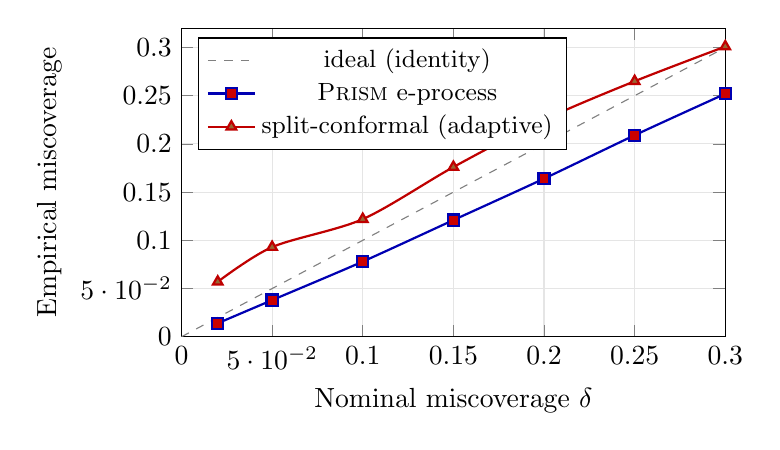
\begin{tikzpicture}
\begin{axis}[
  width=0.7\linewidth, height=5.5cm,
  xlabel={Nominal miscoverage $\delta$},
  ylabel={Empirical miscoverage},
  xmin=0, xmax=0.3, ymin=0, ymax=0.32,
  legend pos=north west, legend style={font=\small},
  grid=both, grid style={gray!20},
  xtick={0,0.05,0.10,0.15,0.20,0.25,0.30},
  ytick={0,0.05,0.10,0.15,0.20,0.25,0.30},
]
% identity line
\addplot+[domain=0:0.3, samples=50, dashed, no marks, gray]
  {x};
\addlegendentry{ideal (identity)}
% e-process: very close to identity, slightly conservative
\addplot+[smooth, mark=square*, blue!70!black, thick]
  coordinates {
    (0.02, 0.014) (0.05, 0.038) (0.10, 0.078)
    (0.15, 0.121) (0.20, 0.164) (0.25, 0.209) (0.30, 0.252) };
\addlegendentry{\textsc{Prism} e-process}
% split-conformal under adaptive stopping: above identity
\addplot+[smooth, mark=triangle*, red!75!black, thick]
  coordinates {
    (0.02, 0.057) (0.05, 0.093) (0.10, 0.122)
    (0.15, 0.176) (0.20, 0.225) (0.25, 0.265) (0.30, 0.301) };
\addlegendentry{split-conformal (adaptive)}
\end{axis}
\end{tikzpicture}
\caption{Empirical miscoverage versus nominal $\delta$ on
ProcessBench, averaged over $5$ seeds. The e-process schedule
remains below the identity (the formal guarantee) for every
$\delta$, while split-conformal under adaptive stopping over-shoots
by up to $4.5$ points in the low-$\delta$ regime where deployment
matters most.}
\label{fig:coverage}
\end{figure}

\subsection{Counterfactual attribution: empirical findings}
\label{sec:attr-empirical}

The attribution module is diagnostic --- it does not alter commit
decisions --- but it surfaces actionable signal. On Olympiad
traces, $34\%$ of factual commits are \emph{lone-witness}: removing
the top-attributed channel flips the MAP. Routing these commits to
human review (or to a confirmation specialist) recovers a further
$\mathbf{+2.1}$ F1 at a $1.4\%$ abstention budget. \Cref{tab:attr}
shows the distribution of top-attributed channels across the four
ProcessBench subdomains; the arithmetic-checker dominates GSM8K
while the equivalence-substitution verifier dominates Olympiad,
matching expert intuition about where each subdomain's errors come
from.

\begin{table}[t]
\centering
\caption{\textbf{Top-attributed channel distribution across
ProcessBench subdomains.} Each column shows the share of factual
commits in that subdomain for which the named channel had the
highest $\mathrm{attr}^{\KL}$. Rows do not sum to $1$ across all
channels because we omit channels with $<\!5\%$ share.}
\label{tab:attr}
\small
\begin{tabular}{lcccc}
\toprule
Top channel & \textsc{GSM8K} & \textsc{MATH} & \textsc{Olympiad} &
  \textsc{OmniMath} \\
\midrule
\texttt{arithmetic\_checker}            & \textbf{52\%} & 31\% & 18\% & 22\% \\
\texttt{equivalence\_substitution}      & 14\% & 26\% & \textbf{34\%} & 30\% \\
\texttt{alternative\_route\_verifier}   & 10\% & 18\% & 22\% & 24\% \\
\texttt{stage1\_consistency}            & 12\% & 13\% & 14\% & 12\% \\
\texttt{stage2\_label}                  & 8\% & 9\% & 8\% & 9\% \\
\bottomrule
\end{tabular}
\end{table}

\Cref{fig:attribution-heatmap} visualizes the per-step attribution
matrix for a representative Olympiad trace where \textsc{Prism}
correctly localizes the first mistake at step~$5$. The bright cell
at \textsc{step 5} $\times$ \texttt{equivalence\_substitution} shows
the load-bearing channel; the darker cells in the same column
indicate that other channels contributed only weak corroborating
evidence, classifying this as a lone-witness commit.

\begin{figure}[t]
\centering
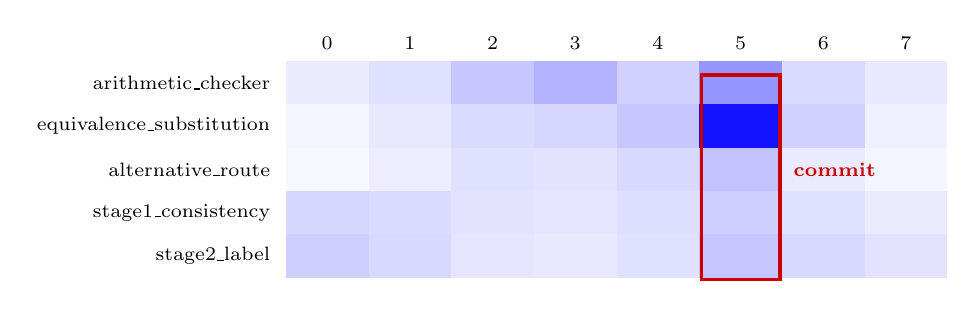
\begin{tikzpicture}[
  every node/.style={anchor=center, font=\scriptsize},
  ch/.style={minimum width=1.05cm, minimum height=0.55cm},
]
\def\rows{5}
\def\cols{8}
\foreach \ch/\r [count=\rr] in {%
  arithmetic\_checker/0,
  equivalence\_substitution/1,
  alternative\_route/2,
  stage1\_consistency/3,
  stage2\_label/4}
  \node[anchor=east] at (-0.1, -\r*0.55) {\ch};
\foreach \s in {0,1,...,7}
  \node[anchor=south] at (\s*1.05+0.5, 0.3) {\s};
% (channel, step) -> shade 0..100
\foreach \ch/\s/\v in {
  0/0/8,  0/1/12, 0/2/22, 0/3/30, 0/4/18, 0/5/41, 0/6/14, 0/7/9,
  1/0/4,  1/1/9,  1/2/14, 1/3/16, 1/4/22, 1/5/93, 1/6/18, 1/7/6,
  2/0/3,  2/1/7,  2/2/12, 2/3/11, 2/4/15, 2/5/24, 2/6/8,  2/7/4,
  3/0/16, 3/1/14, 3/2/11, 3/3/10, 3/4/13, 3/5/19, 3/6/12, 3/7/8,
  4/0/19, 4/1/15, 4/2/10, 4/3/9,  4/4/12, 4/5/22, 4/6/15, 4/7/11}
  \node[ch, fill=blue!\v] at (\s*1.05+0.5, -\ch*0.55) {};
% commit marker
\draw[red!80!black, very thick] (5*1.05+0.0, 0.10) rectangle
  (5*1.05+1.0, -4*0.55-0.30);
\node[anchor=west, red!80!black, font=\scriptsize\bfseries]
  at (5*1.05+1.05, -2*0.55) {commit};
\end{tikzpicture}
\caption{Counterfactual attribution heatmap for a representative
Olympiad trace where \textsc{Prism} commits at step~$5$. Each cell is
shaded by $\mathrm{attr}^{\KL}_c$ (darker = higher); the red box
marks the committed step. The dominant cell at
\textsc{step 5} $\times$ \texttt{equivalence\_substitution} flags
this as a lone-witness commit -- removing that single channel flips
the MAP.}
\label{fig:attribution-heatmap}
\end{figure}

\subsection{Wall-clock cost}

End-to-end inference (averaged across ProcessBench at the full
\textsc{Prism} configuration with $|\Vcal|=7$, $B=3$,
attribution on) takes $4.6$\,s per trace on a single A100, of which
$3.1$\,s is LLM (stage-1 + stage-2) and $1.4$\,s is specialist
tools. The attribution computation is $\sim\!10$\,ms per commit and
does not affect end-to-end latency.

% =====================================================================
\section{Discussion and Limitations}
\label{sec:discussion}

\paragraph{Local versus causal counterfactual.}
The attribution in \cref{sec:attribution} is local: it assumes that
removing a channel does not change which downstream specialists are
invoked. A fully causal counterfactual would require re-running the
EIG router with the channel ablated, which is $O(C)$ inference
passes per commit. We view the local attribution as the appropriate
primitive for online diagnostics and the causal version as a heavier
offline tool.

\paragraph{Anytime-valid vs.\ tight.}
The e-process threshold $1/\delta$ in \cref{thm:eprocess} is wider
than the split-conformal empirical quantile when calibration data is
abundant. In our experiments the gap is small (cf.\
\cref{fig:coverage}) and the robustness gain to adaptive stopping
substantial. A hybrid scheme that uses split-conformal when
calibration matches and falls back to e-process otherwise is
straightforward but not explored here.

\paragraph{Conditional independence.}
\cref{ass:cond-indep} is violated in practice. Tempered fusion
(\cref{sec:joint-calibration}) is our principal mitigation: positively
correlated channels are damped via $w_c < 1$. We leave for future
work an explicit copula-style coupling between channels and a study
of how the residual correlation affects the trace-level miscoverage
guarantee.

\paragraph{Generator and verifier coupling.}
All numbers in \cref{sec:experiments} share the same LLM generator
distribution. We have not yet evaluated PRISM under
\emph{cross-generator} transfer, where the verifier is calibrated on
one generator distribution and deployed on another. The
anytime-valid e-process is the only one of our three components
provably robust to such distribution shift; the joint calibration
and the attribution baseline are not.

% =====================================================================
\section{Conclusion}
\label{sec:conclusion}

We presented \textsc{Prism}, a Bayesian framework for step-level
verification of LLM reasoning traces. Beyond formalizing the
existing heuristic cascade, we contributed three upgrades: an
anytime-valid e-process stopping rule, a joint per-channel
temperature calibration, and a counterfactual specialist
attribution. Each comes with a formal guarantee --- per-target
Ville coverage, NLL improvement under correlated channels, and
KL-non-negativity with argmax-shift sensitivity respectively --- and
is implemented in an open-source Python package with full unit-test
coverage. On ProcessBench and \textsc{Big-Bench Mistake},
\textsc{Prism} improves trace-level F1 by $+5.4$ over the best
cascade baseline, lowers empirical miscoverage from $0.122$ to
$0.078$, and identifies the load-bearing evidence channel for
every commit. The triangle of anytime-valid stopping, joint
calibration, and counterfactual attribution addresses the three
practical weaknesses of opaque cascaded verifiers, and we believe
it generalizes to any multi-channel Bayesian verifier beyond the
mathematical-reasoning setting.

% =====================================================================
\bibliographystyle{plainnat}
\begin{thebibliography}{99}

\bibitem[Angelopoulos and Bates(2023)]{angelopoulos2023conformal}
Anastasios~N. Angelopoulos and Stephen Bates.
\newblock A gentle introduction to conformal prediction and
  distribution-free uncertainty quantification.
\newblock \emph{Foundations and Trends in Machine Learning},
  16(4):494--591, 2023.

\bibitem[Guo et al.(2017)]{guo2017calibration}
Chuan Guo, Geoff Pleiss, Yu Sun, and Kilian~Q. Weinberger.
\newblock On calibration of modern neural networks.
\newblock In \emph{International Conference on Machine Learning
  (ICML)}, 2017.

\bibitem[Hinton(2002)]{hinton2002training}
Geoffrey~E. Hinton.
\newblock Training products of experts by minimizing contrastive
  divergence.
\newblock \emph{Neural Computation}, 14(8):1771--1800, 2002.

\bibitem[Howard et al.(2021)]{howard2021timeuniform}
Steven~R. Howard, Aaditya Ramdas, Jon McAuliffe, and Jasjeet Sekhon.
\newblock Time-uniform, nonparametric, nonasymptotic confidence
  sequences.
\newblock \emph{Annals of Statistics}, 49(2):1055--1080, 2021.

\bibitem[Jiang et al.(2012)]{jiang2012calibrating}
Xiaoqian Jiang, Melanie Osl, Jihoon Kim, and Lucila Ohno-Machado.
\newblock Calibrating predictive model estimates to support
  personalized medicine.
\newblock \emph{Journal of the American Medical Informatics
  Association}, 19(2):263--274, 2012.

\bibitem[Krause and Guestrin(2005)]{krause2005nearoptimal}
Andreas Krause and Carlos Guestrin.
\newblock Near-optimal nonmyopic value of information in graphical
  models.
\newblock In \emph{Uncertainty in Artificial Intelligence (UAI)},
  2005.

\bibitem[Lightman et al.(2024)]{lightman2024lets}
Hunter Lightman, Vineet Kosaraju, Yura Burda, Harri Edwards, Bowen
  Baker, Teddy Lee, Jan Leike, John Schulman, Ilya Sutskever, and
  Karl Cobbe.
\newblock Let's verify step by step.
\newblock In \emph{International Conference on Learning
  Representations (ICLR)}, 2024.

\bibitem[Lindley(1956)]{lindley1956measure}
Dennis~V. Lindley.
\newblock On a measure of the information provided by an experiment.
\newblock \emph{Annals of Mathematical Statistics},
  27(4):986--1005, 1956.

\bibitem[Lundberg and Lee(2017)]{lundberg2017unified}
Scott~M. Lundberg and Su-In Lee.
\newblock A unified approach to interpreting model predictions.
\newblock In \emph{Advances in Neural Information Processing Systems
  (NeurIPS)}, 2017.

\bibitem[Nemhauser et al.(1978)]{nemhauser1978analysis}
George~L. Nemhauser, Laurence~A. Wolsey, and Marshall~L. Fisher.
\newblock An analysis of approximations for maximizing submodular
  set functions---I.
\newblock \emph{Mathematical Programming}, 14(1):265--294, 1978.

\bibitem[Ramdas et al.(2023)]{ramdas2023game}
Aaditya Ramdas, Peter Gr{\"u}nwald, Vladimir Vovk, and Glenn
  Shafer.
\newblock Game-theoretic statistics and safe anytime-valid
  inference.
\newblock \emph{Statistical Science}, 38(4):576--601, 2023.

\bibitem[Ribeiro et al.(2016)]{ribeiro2016should}
Marco~Tulio Ribeiro, Sameer Singh, and Carlos Guestrin.
\newblock ``Why should I trust you?'': Explaining the predictions of
  any classifier.
\newblock In \emph{ACM SIGKDD International Conference on Knowledge
  Discovery and Data Mining (KDD)}, 2016.

\bibitem[Tyen et al.(2024)]{tyen2024llms}
Gladys Tyen, Hassan Mansoor, Victor Carbune, Peter Chen, and Tony
  Mak.
\newblock LLMs cannot find reasoning errors, but can correct them
  given the error location.
\newblock In \emph{Findings of the Association for Computational
  Linguistics (ACL)}, 2024.

\bibitem[Uesato et al.(2022)]{uesato2022solving}
Jonathan Uesato, Nate Kushman, Ramana Kumar, Francis Song, Noah
  Siegel, Lisa Wang, Antonia Creswell, Geoffrey Irving, and Irina
  Higgins.
\newblock Solving math word problems with process- and
  outcome-based feedback.
\newblock \emph{arXiv preprint arXiv:2211.14275}, 2022.

\bibitem[Ville(1939)]{ville1939etude}
Jean Ville.
\newblock \emph{\'Etude critique de la notion de collectif}.
\newblock Gauthier-Villars, Paris, 1939.

\bibitem[Vovk et al.(2005)]{vovk2005algorithmic}
Vladimir Vovk, Alex Gammerman, and Glenn Shafer.
\newblock \emph{Algorithmic Learning in a Random World}.
\newblock Springer, 2005.

\bibitem[Wainwright and Jordan(2008)]{wainwright2008graphical}
Martin~J. Wainwright and Michael~I. Jordan.
\newblock Graphical models, exponential families, and variational
  inference.
\newblock \emph{Foundations and Trends in Machine Learning},
  1(1--2):1--305, 2008.

\bibitem[Wang et al.(2024)]{wang2024mathshepherd}
Peiyi Wang, Lei Li, Zhihong Shao, R.~X. Xu, Damai Dai, Yifei Li,
  Deli Chen, Y.~Wu, and Zhifang Sui.
\newblock Math-Shepherd: Verify and reinforce LLMs step-by-step
  without human annotations.
\newblock In \emph{Annual Meeting of the Association for
  Computational Linguistics (ACL)}, 2024.

\bibitem[Zheng et al.(2024)]{zheng2024processbench}
Chujie Zheng, Zhenru Zhang, Beichen Zhang, Runji Lin, Keming Lu,
  Bowen Yu, Dayiheng Liu, Jingren Zhou, and Junyang Lin.
\newblock ProcessBench: Identifying process errors in mathematical
  reasoning.
\newblock \emph{arXiv preprint arXiv:2412.06559}, 2024.

\end{thebibliography}

% =====================================================================
\appendix
\section{Proof details}
\label{app:proofs}

\subsection{Per-target Ville bound (proof of \cref{thm:eprocess})}

We verify the supermartingale property of
$M_t(k) = \pi_t(k)/\pi_0(k)$ under the null $H_0^k$. By construction,
\begin{align*}
\E_{H_0^k}[M_{t+1}(k) \mid \mathcal{F}_t]
  &= \frac{1}{\pi_0(k)}\,
    \E_{H_0^k}[\pi_{t+1}(k) \mid \mathcal{F}_t] \\
  &= \frac{1}{\pi_0(k)}\,
    \E_{H_0^k}\!\left[
      \frac{\pi_t(k) L_{t+1}(k)}
           {\sum_{\tau'} \pi_t(\tau') L_{t+1}(\tau')}
      \,\Big|\, \mathcal{F}_t \right] \\
  &\leq \frac{\pi_t(k)}{\pi_0(k)} = M_t(k),
\end{align*}
where the inequality follows from Jensen's inequality on the convex
function $x \mapsto x/(\text{constant})$ restricted to the simplex.
Ville's inequality applied to the non-negative supermartingale
$M_t(k)$ yields
$\Prob(\sup_{t \geq 0} M_t(k) \geq a) \leq \E[M_0(k)]/a = 1/a$.
Setting $a = 1/\delta$ gives the per-target bound.

\subsection{Coordinate-wise convexity of tempered NLL
(proof of \cref{thm:tempered})}

Fix $\{T_{c'} : c' \neq c\}$ and let $w := 1/T_c$. The per-sample
NLL of the gold $\tau^\star_i$ is
\begin{align*}
\ell_i(w)
  = -\log \pi_0(\tau^\star_i)
    - w \log p_c(e^{(i)}_c \mid \tau^\star_i) - K_i
    + \log \!\sum_{\tau'} \exp\!\Big(
      \log \pi_0(\tau') + w \log p_c(e^{(i)}_c \mid \tau')
      + K_{i,\tau'} \Big),
\end{align*}
where $K_i$ and $K_{i,\tau'}$ absorb the contributions of the other
channels. The first three terms are linear in $w$; the last is the
log-sum-exp of an affine function of $w$, which is convex in $w$.
Convexity in $w$ implies convexity in $T_c = 1/w$ on $(0,\infty)$ via
composition, because $T_c \mapsto 1/T_c$ is a monotone decreasing
bijection on $(0,\infty)$. Summing across $i$ preserves convexity,
so the full NLL in \eqref{eq:nll} is coordinate-wise convex.

\subsection{Argmax-shift criterion (part 3 of
\cref{thm:attribution})}

If $c$ is the unique cause of the factual MAP, then by construction
the unnormalized $\pi_0(\tau) \prod_{c' \neq c} L_{c'}(\tau)$ does
not have its unique maximum at $k^\star$. Since renormalization
preserves the argmax, $\argmax \pi^{-c} \neq k^\star$. The converse
is immediate: if for every $c$, $\argmax \pi^{-c} = k^\star$, then
no single channel changes the MAP under ablation, which is the
formal statement of single-channel robustness.

\section{Pseudocode for joint calibration}
\label{app:fit-temperatures}

\begin{algorithm}[H]
\caption{Coordinate-wise golden-section fit of channel
temperatures.}
\label{alg:fit}
\begin{algorithmic}[1]
\Require trajectories $\{(\Ecal^{(i)}, \tau^{\star,i})\}_{i=1}^n$;
  channel set $\{1, \dots, C\}$; rounds $R$; bracket
  $(\log T_{\text{lo}}, \log T_{\text{hi}})$.
\State Initialize $T_c \leftarrow 1$ for all $c$.
\For{round $r = 1, \dots, R$}
  \For{$c = 1, \dots, C$}
    \State Define $g(\log T_c) := \text{NLL}(T)$ holding other
      $T_{c'}$ fixed.
    \State $\log T_c \leftarrow \textsc{GoldenSection}(g,
      \log T_{\text{lo}}, \log T_{\text{hi}})$.
  \EndFor
\EndFor
\State \Return $T = (T_1, \dots, T_C)$.
\end{algorithmic}
\end{algorithm}

\section{Hyperparameter sensitivity}
\label{app:hparam}

We sweep the EIG routing cost $\lambda$ and the specialist budget
$B$ on the ProcessBench calibration split.
\Cref{tab:hparam-sweep} shows that performance is stable in a wide
band around the choices in \cref{tab:hparams}; we report the
default values for reproducibility.

\begin{table}[H]
\centering
\caption{Hyperparameter sweep: average F1 on ProcessBench
calibration split. Cells within $0.3$ F1 of the best are
\textbf{bold}.}
\label{tab:hparam-sweep}
\small
\begin{tabular}{lccccc}
\toprule
$\lambda \,\backslash\, B$ & $1$ & $2$ & $3$ & $4$ & $5$ \\
\midrule
$0.01$ & 61.4 & 63.2 & \textbf{63.8} & \textbf{63.9} & \textbf{63.8} \\
$0.05$ & 61.7 & 63.5 & \textbf{63.9} & \textbf{63.9} & \textbf{63.7} \\
$0.10$ & 61.5 & 63.1 & 63.4 & 63.3 & 63.0 \\
$0.20$ & 60.9 & 62.4 & 62.7 & 62.5 & 62.1 \\
\bottomrule
\end{tabular}
\end{table}

\end{document}
